\RequirePackage{plautopatch}
\documentclass{jlreq}

\usepackage{aliascnt}
\usepackage{amsmath,amssymb,amsthm}
\usepackage{anyfontsize}
\usepackage[backend=biber,style=alphabetic,]{biblatex}
\usepackage{bm,bbm}
\usepackage{cancel}
\usepackage{color}
\usepackage{fancyvrb}
\usepackage{fontspec}
\usepackage{mathrsfs}
\usepackage{mathtools}
\usepackage{siunitx,physics}
\usepackage{url}
\usepackage{tikz}

% "Make sure it comes last of your loaded packages."
\usepackage[luatex,unicode,hidelinks,pdfusetitle]{hyperref}

% biblatex
\addbibresource{refs.bib}


% tikz
\usetikzlibrary{perspective}
\usetikzlibrary{decorations.markings}

% https://tex.stackexchange.com/a/39282
\tikzset{->-/.style={decoration={
  markings,
  mark=at position 0.65 with {\arrow{>}}},postaction={decorate}}
}

\title{本間・五十嵐・川口『数値電磁力学』 (5.51)式の導出}
\author{hnagamin\thanks{\url{https://www.downcastingsoft.net/7e5/diary/article/2022/05/28/hik02-whitney/}}}

\allowdisplaybreaks

\begin{document}

\maketitle

体積座標\(\lambda_k\)とその勾配\(\nabla\lambda_k\)は教科書~(5.49), (5.50)式で以下のように与えられていた\cite[p. 159]{Homma2002}.
ここで,\(v\)は四面体の体積である.
\begin{align}
  \lambda_k
  &= \frac{1}{6v}(\bm{x}-\bm{x}_m)\cdot(\bm{x}_{l n}\times\bm{x}_{lm})
  \label{eq:lambdak} \\
  \nabla \lambda_k
  &= \frac{1}{6v}\bm{x}_{l n}\times\bm{x}_{lm}
  \label{eq:dlambdak}
\end{align}

初めに,\(\lambda_l\)とその勾配\(\nabla\lambda_l\)の表式を求める.
そのためには,\eqref{eq:lambdak},~\eqref{eq:dlambdak}式で添字を\(
  (k,l,m,n)\mapsto(l,m,k,n)
\)と置換すればよい.

\begin{align}
  \lambda_l
  &= \frac{1}{6v}(\bm{x}-\bm{x}_k)\cdot(\bm{x}_{mn}\times\bm{x}_{mk})
  \label{eq:lambdal} \\
  \nabla\lambda_l
  &= \frac{1}{6v}\bm{x}_{mn}\times\bm{x}_{mk}
  \label{eq:dlambdal}
\end{align}

\begin{figure}
  \centering
  \begin{tabular}{c}
    \begin{minipage}{0.48\linewidth}
      \centering
      % https://tex.stackexchange.com/a/174424
      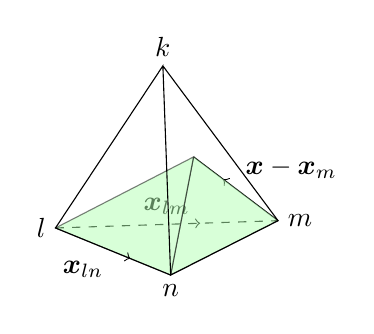
\begin{tikzpicture}[3d view={-47}{70}]
        \coordinate[label=above:{\(k\)}] (A) at (+1,+1,+1);
        \coordinate[label=below:{\(n\)}] (B) at (-1,-1,+1);
        \coordinate[label=right:{\(m\)}] (C) at (+1,-1,-1);
        \coordinate[label=left:{\(l\)}] (D) at (-1,+1,-1);
        \coordinate (X) at (0.5, 0, 0.5);

        \draw[dashed,->-] (D) -- (C) node[midway,above] {\(\bm{x}_{lm}\)};
        \draw[->-] (C) -- (X) node[midway,above right] {\(\bm{x}-\bm{x}_m\)};
        \draw[fill=green!30, opacity=0.5] (X) -- (B) -- (C);
        \draw[fill=green!30, opacity=0.5] (X) -- (B) -- (D) -- cycle;
        \draw[->-] (D) -- (B) node[midway, below left] {\(\bm{x}_{l n}\)};
        \draw (D) -- (A) -- (B) -- (C) -- (A);
      \end{tikzpicture}
      \caption{四面体\(klmn\)}
    \end{minipage}
    \hfill
    \begin{minipage}{0.48\linewidth}
      \centering
      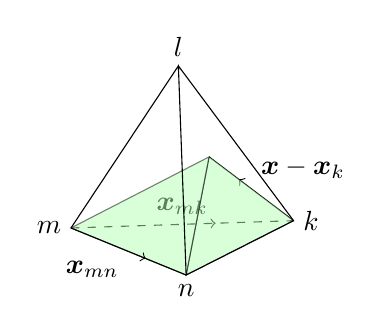
\begin{tikzpicture}[3d view={-47}{70}]
        \coordinate[label=above:{\(l\)}] (A) at (+1,+1,+1);
        \coordinate[label=below:{\(n\)}] (B) at (-1,-1,+1);
        \coordinate[label=right:{\(k\)}] (C) at (+1,-1,-1);
        \coordinate[label=left:{\(m\)}] (D) at (-1,+1,-1);
        \coordinate (X) at (0.5, 0, 0.5);

        \draw[dashed,->-] (D) -- (C) node[midway,above] {\(\bm{x}_{mk}\)};
        \draw[->-] (C) -- (X) node[midway,above right] {\(\bm{x}-\bm{x}_k\)};
        \draw[fill=green!30, opacity=0.5] (X) -- (B) -- (C);
        \draw[fill=green!30, opacity=0.5] (X) -- (B) -- (D) -- cycle;
        \draw[->-] (D) -- (B) node[midway, below left] {\(\bm{x}_{m n}\)};
        \draw (D) -- (A) -- (B) -- (C) -- (A);
      \end{tikzpicture}
      \caption{四面体\(lmkn\)}
    \end{minipage}
  \end{tabular}
\end{figure}

~\eqref{eq:lambdak},~\eqref{eq:dlambdak},~\eqref{eq:lambdal},~\eqref{eq:dlambdal}式より,次の等式が成り立つ.
\begin{align}
  \lambda_k
  &= (\bm{x}-\bm{x}_m)\cdot\nabla\lambda_k
  \label{eq:lk-dlk} \\
  \lambda_l
  &= (\bm{x}-\bm{x}_k)\cdot\nabla\lambda_l
  \label{eq:ll-dll}
\end{align}

次に,ベクトル三重積の公式(BAC-CAB rule)を確認する.
三次元ベクトル\(\bm{a},\bm{b},\bm{c}\)に対し,以下の等式が成り立つ\cite[p. 237]{Homma2002}.
\begin{align}
  \bm{a}\times(\bm{b}\times\bm{c})
  &= (\bm{a}\cdot\bm{c})\bm{b}-(\bm{a}\cdot\bm{b})\bm{c}
  \label{eq:bac-cab} \\
  (\bm{a}\times\bm{b})\times\bm{c}
  &= (\bm{a}\cdot\bm{c})\bm{b}-(\bm{b}\cdot\bm{c})\bm{a}
  \label{eq:bac-abc}
\end{align}

以上をふまえると,辺\(e=\left\{k,l\right\}\)に関する1次ホイットニー要素基底\(\bm{w}_{e}\)は次のように書ける.
\begin{align}
  \bm{w}_e
  &= \lambda_k \nabla\lambda_l - \lambda_l \nabla\lambda_k \\
  &= [(\bm{x}-\bm{x}_m)\cdot\nabla\lambda_k]\nabla\lambda_l
    -[(\bm{x}-\bm{x}_k)\cdot\nabla\lambda_l]\nabla\lambda_k
    & &\text{\eqref{eq:lk-dlk},~\eqref{eq:ll-dll}式} \\
  &= [(\bm{x}-\bm{x}_m)\cdot\nabla\lambda_k]\nabla\lambda_l
    -[(\bm{x}-\bm{x}_m)\cdot\nabla\lambda_l]\nabla\lambda_k
    -[(\bm{x}_m-\bm{x}_k)\cdot\nabla\lambda_l]\nabla\lambda_k \\
  &= (\bm{x}-\bm{x}_m)\times(\nabla\lambda_l\times\nabla\lambda_k)
    -\cancel{(\bm{x}_{km}\cdot\nabla\lambda_l)}\nabla\lambda_k
    & &\text{\eqref{eq:bac-cab}式} \\
  &= (\bm{x}-\bm{x}_m)\times(\nabla\lambda_l\times\nabla\lambda_k)
    & &\bm{x}_{km}\perp \nabla\lambda_l
    \label{eq:we}
\end{align}

一方,\eqref{eq:dlambdal}式と\eqref{eq:bac-abc}式より\(\nabla\lambda_l\times\nabla\lambda_k\)は次のように表される.
\begin{align}
  \nabla\lambda_l \times \nabla\lambda_k
  &= \frac{1}{6v} (\bm{x}_{mn}\times\bm{x}_{mk})\times\nabla\lambda_k \\
  &= \frac{1}{6v}
      \left[
        (\bm{x}_{mn}\cdot\nabla\lambda_k)\bm{x}_{mk}
       -(\bm{x}_{mk}\cdot\nabla\lambda_k)\bm{x}_{mn}
      \right]
\end{align}
最右辺第2項に注目すると,\(\nabla\lambda_k\)は平面\(lnm\)に垂直だから\(\bm{x}_{mn}\cdot\nabla\lambda_k=0\)である.
一方第1項において,スカラー三重積の性質から次が分かる.
\begin{align}
  \bm{x}_{mk}\cdot\nabla\lambda_k
  &= \frac{1}{6v}\bm{x}_{mk}\cdot(\bm{x}_{l n}\times\bm{x}_{lm})
  = 1
\end{align}
以上より
\begin{align}
  \bm{w}_e
  &= (\bm{x}-\bm{x}_m)\times\frac{1}{6v}[0\bm{x}_{mk}-1\bm{x}_{mn}]
  = \frac{1}{6v}(\bm{x}_m-\bm{x})\times\bm{x}_{mn}
\end{align}
であり,教科書~(5.51)式が導かれた.

\printbibliography[title={参考文献}]

\end{document}
